\begin{center}
\textbf{\Large Геометрический разнобой}\\
%\textit{Профи}\\
\textit{21.07.16}
\end{center}

\renewcommand{\epigraphwidth}{.55\textheight}
\epigraph{\it искренне не понимаю чьего-либо негодования по поводу третьей геометрии на межнаре}{А. Семченков}

\begin{problems}
\item Квадраты $ABCD$ и $CPQR$ одинаково ориентированы (см. рис.) и имеют только одну общую точку (точку $C$). Докажите, что $BR=DP$.
%нужна картинка!!!!

\item Дан выпуклый четырёхугольник, у которого нет параллельных сторон. Где находится такая точка, которая одновременно равноудалена от двух пар его противоположных сторон? Сколько может быть таких точек?
%желательна картинка

\begin{center}
	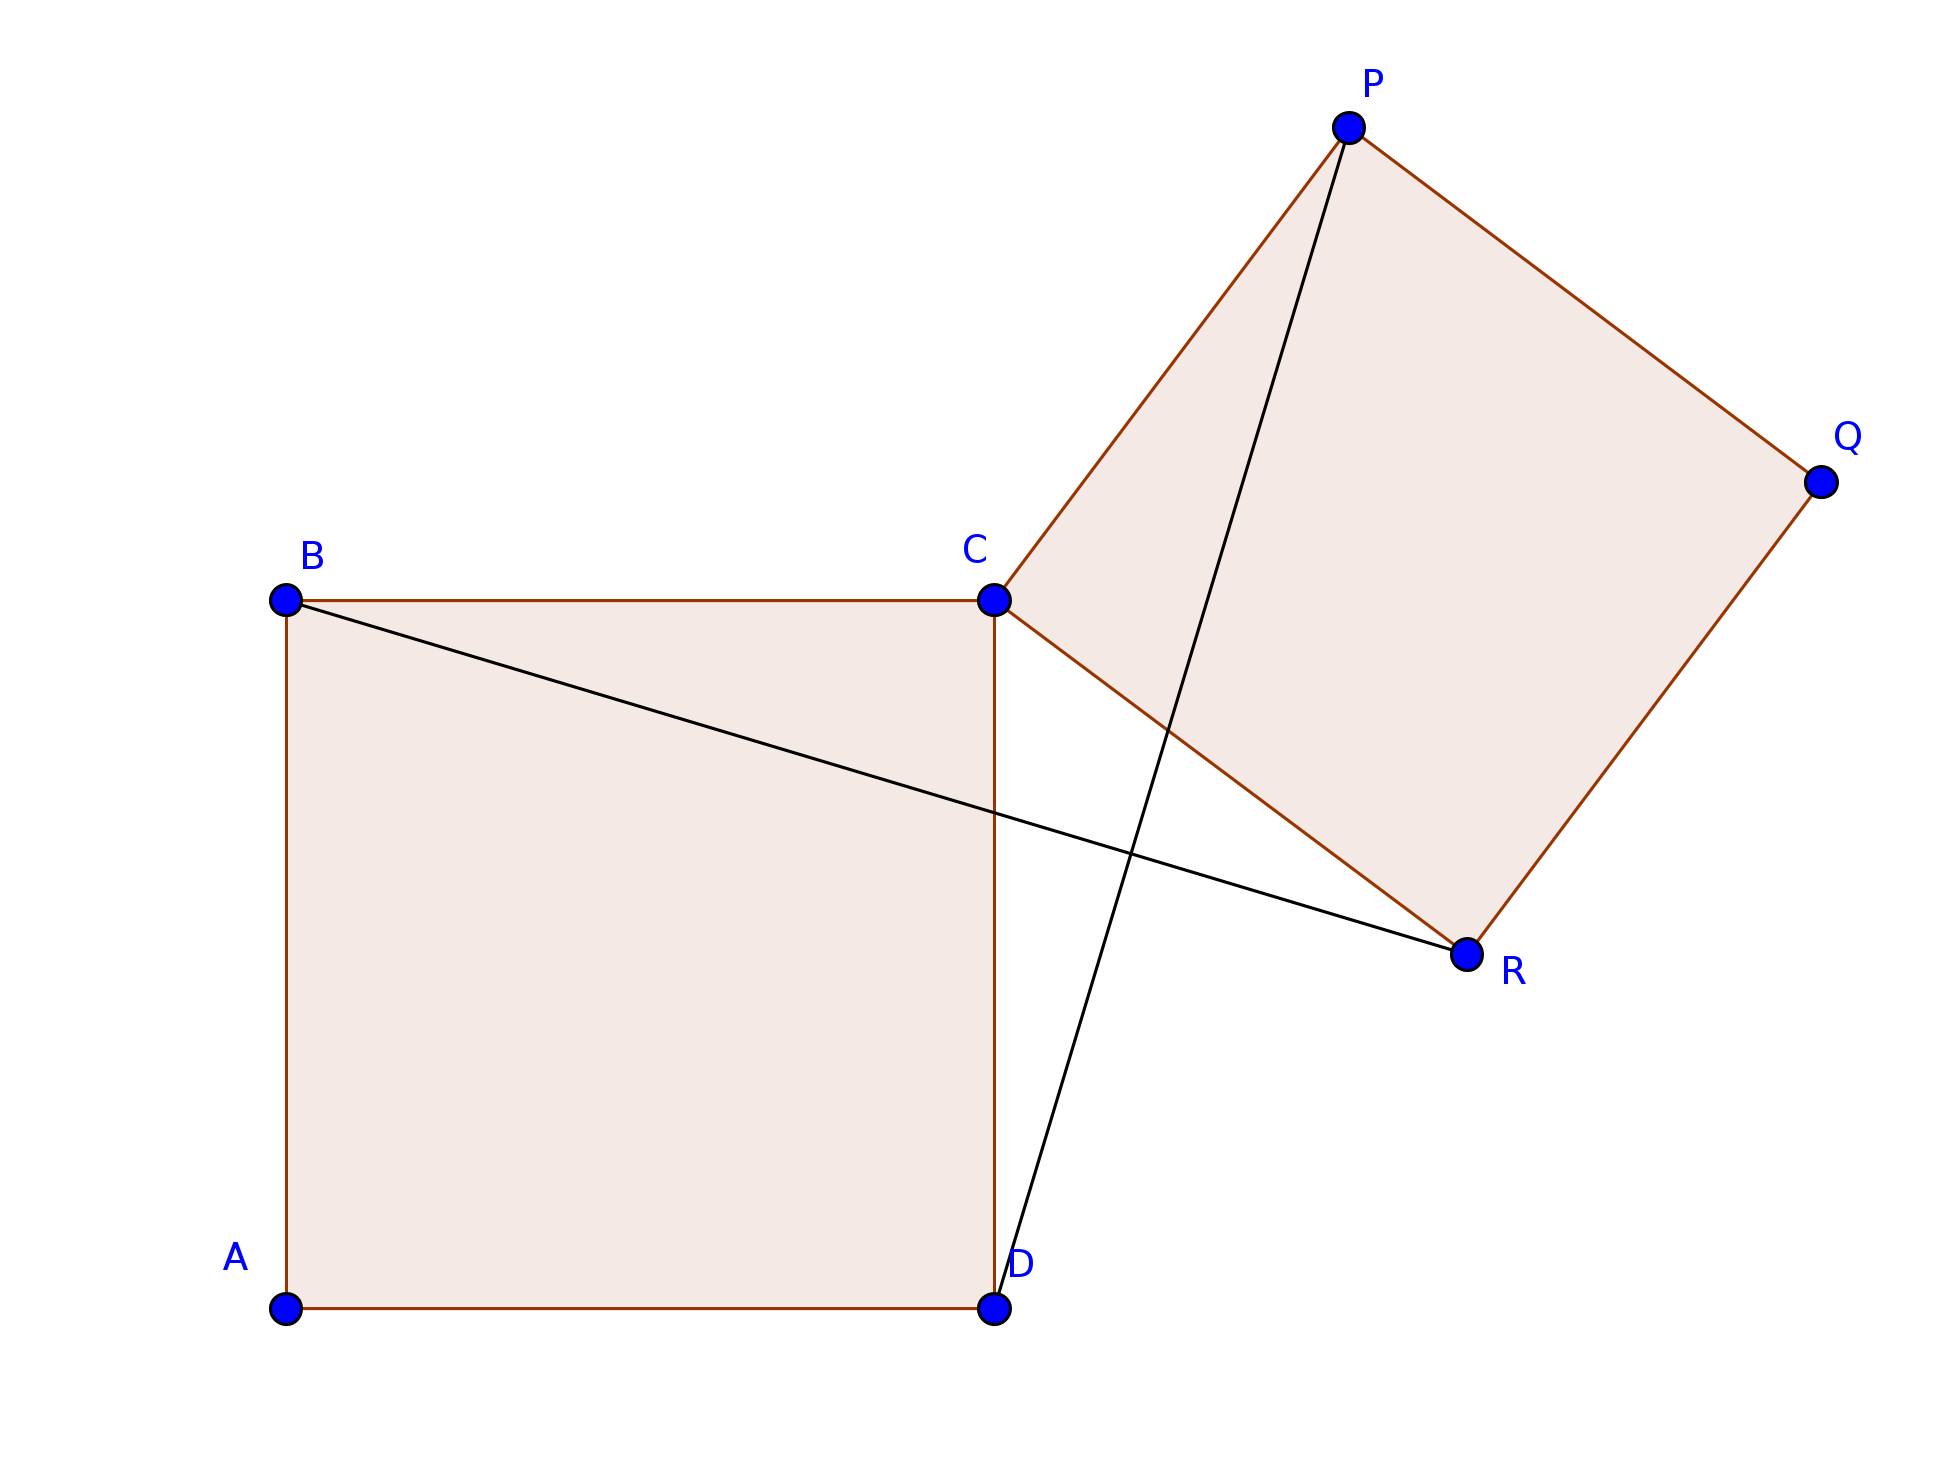
\includegraphics[width=.45\textwidth]{georazn01}
	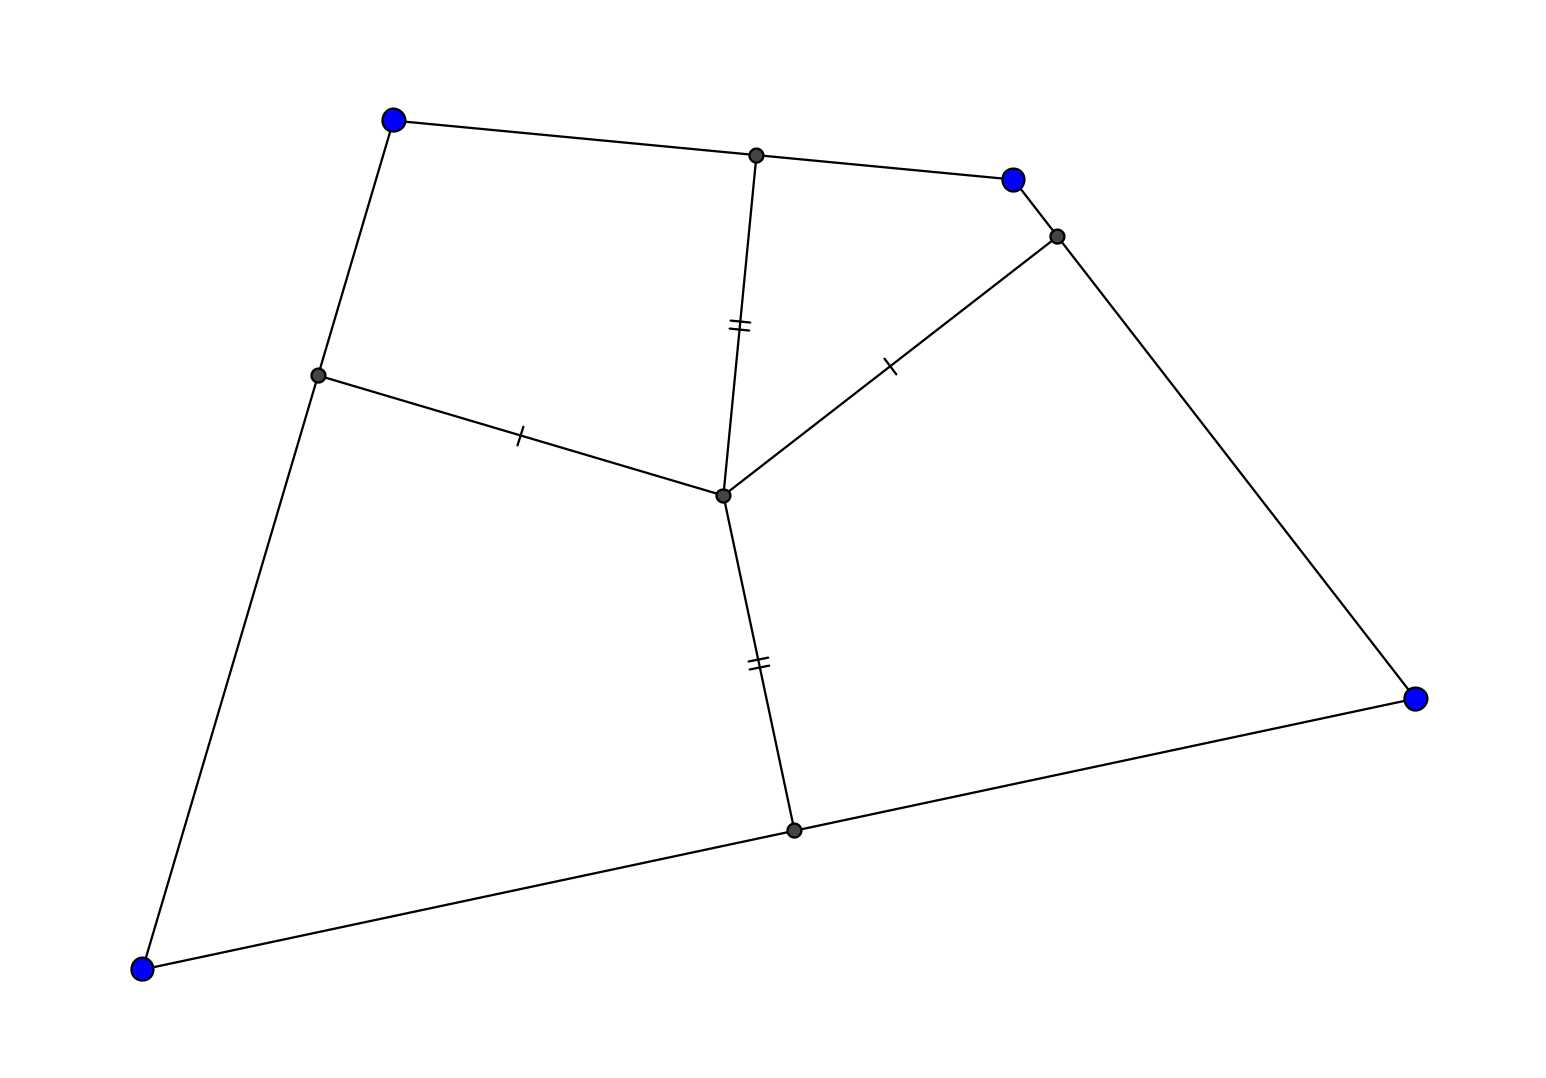
\includegraphics[width=.45\textwidth]{georazn02}
\end{center}

\item На стороне $BC$ квадрата $ABCD$ выбрана точка $M$. На стороне $CD$ выбрана такая точка $P$, что $AP\perp MD$. На стороне $AB$ выбрана такая точка $Q$, что $DQ\perp MA$. Докажите, что прямая $PQ$ проходит через центр квадрата.
%симметричная картинка

\item Бильярд имеет форму остроугольного треугольника $ABC$. Из точки $K$ стороны $AB$ выпустили бильярдный шар, который отразился (по правилу угол падения равен углу отражения) в точках $L, M$ от сторон $BC, CA$, возвратился в точку $K$ и вновь вышел на траекторию $KLM$. Докажите, что точки $K, L, M$~--- точки основания высот треугольника $ABC$.

\item Внутри острого угла $XOY$ взяты точки $M$ и $N$ так, что $\angle XON = \angle YOM$. На отрезке $OX$ выбирается точка $Q$ так, что $\angle NQO = \angle MQX$, а на отрезке $OY$ выбирается точка $P$ так, что $\angle NPO = \angle MPY$. Докажите, что длины ломаных $MPN$ и $MQN$ равны.

\item В треугольнике $ABC$ на сторонах $AC$ и $BC$ взяты точки $X$ и $Y$ такие, что $\angle ABX = \angle YAC$, $\angle AYB = \angle BXC$, $XC = YB$. Найдите углы треугольника $ABC$.
% 4 признак + небольшой счёт углов

\item На~сторонах $AB$ и~$AD$ квадрата $ABCD$ выбраны точки $N$ и~$P$ соответственно,
а~на~отрезке~$AN$ выбрана точка~$Q$ так, что $NP = NC$
и~$\angle QPN = \angle NCB$.
Докажите, что $\angle BCQ = \frac{1}{2} \angle AQP$.

%\item Даны два выпуклых многоугольника $A_1A_2A_3A_4...A_n$ и $B_1B_2B_3B_4...B_n$. Известно, что $A_1A_2 = B_1B_2$, $A_2A_3 = B_2B_3,..., A_nA_1 = B_nB_1$ и $n - 3$ угла одного многоугольника равны соответственным углам другого. Будут ли многоугольники равны?

\end{problems}